\documentclass[11pt]{article}

\usepackage[utf8]{inputenc}
\usepackage[T1]{fontenc}
\usepackage{lmodern}
\usepackage{geometry}
\geometry{margin=1in}
\usepackage{amsmath,amssymb,amsfonts,amsthm,mathtools,bm}
\usepackage{physics}
\usepackage{tikz}
\usetikzlibrary{arrows.meta,positioning,calc,decorations.pathmorphing,patterns}
\usepackage{hyperref}
\usepackage{enumitem}
\usepackage{authblk}

\hypersetup{colorlinks=true,linkcolor=blue,citecolor=blue,urlcolor=blue}

\newtheorem{theorem}{Theorem}
\newtheorem{proposition}{Proposition}
\newtheorem{lemma}{Lemma}
\newtheorem{definition}{Definition}
\newtheorem{corollary}{Corollary}
\theoremstyle{remark}
\newtheorem{remark}{Remark}

\title{Particle-ness as a Continuous Spectral Observability Functional}
\author{Author Name}
\affil{Independent Research Draft}
\date{Draft \today}

\begin{document}
\maketitle

\begin{abstract}
Standard quantum field theory distinguishes asymptotic on-shell particles from off-shell internal excitations, resonances, and continuum states. In informal language this becomes a binary distinction between ``real'' and ``virtual'' particles. This paper introduces a mathematical refinement: particle-like behavior can be represented by a continuous \emph{spectral observability functional} built from the K\"allen--Lehmann spectral density, detector resolution, finite observation time, and effective decay width. The framework preserves the sharp LSZ distinction for exact asymptotic states while adding a quantitative scale for how particle-like an excitation is to a finite detector. We prove boundedness, monotonicity under observation time, the stable-pole limit, and suppression of broad resonances. The result is not an ontological claim that virtual particles are ordinary particles; it is a formal proposal that empirical particle-ness is a continuous emergent property of field spectral structure.
\end{abstract}

\tableofcontents

\section{Introduction}

Particle language is indispensable in quantum field theory (QFT), yet it is not fundamental in the same way as fields and correlation functions. Stable asymptotic particles are associated with poles of correlation functions and LSZ scattering states. Unstable resonances correspond to broadened structures or complex poles. Multiparticle states generate continua and branch cuts. Virtual particles appear as internal lines in perturbative expansions, not as directly detectable asymptotic objects.

The common words ``real'' and ``virtual'' can obscure this layered structure. This paper introduces a new way to look at the problem: keep the sharp formal categories of QFT, but define a continuous score measuring how particle-like a spectral excitation appears to a finite-resolution detector.

\paragraph{Core proposal.} Let $\rho(\mu^2)$ be a spectral density, $K_D(\mu^2)$ a detector kernel, $T$ an observation time, and $\Gamma(\mu^2)$ an effective width or decoherence/decay rate. Define
\begin{equation}
\mathcal P_T[\rho,K_D,\Gamma]
= \frac{\int_0^\infty \rho(\mu^2)K_D(\mu^2)e^{-T\Gamma(\mu^2)}\,d\mu^2}
{\int_0^\infty \rho(\mu^2)K_D(\mu^2)\,d\mu^2},
\end{equation}
when the denominator is nonzero. The number $\mathcal P_T\in[0,1]$ is called the \emph{spectral observability} or \emph{particle-ness} score.

\section{Literature grounding}

The K\"allen--Lehmann representation expresses two-point functions as spectral integrals over positive spectral weights under standard assumptions. LSZ reduction relates isolated one-particle poles to asymptotic scattering amplitudes. Resonance theory shows that unstable particles are not exact asymptotic states, but can behave particle-like for finite time and finite energy resolution. Detector models, including Unruh--DeWitt detectors, emphasize that observed particle content depends on detector coupling, trajectory, bandwidth, and time window.

This paper builds from those ideas but adds one object: a normalized functional designed to quantify particle-like observability continuously.

\section{Spectral preliminaries}

Consider a scalar field $\phi$ in a relativistic QFT. Under standard Wightman axioms, the time-ordered two-point function admits a spectral representation
\begin{equation}
G_F(p^2)=\int_0^\infty d\mu^2\,\rho(\mu^2)\frac{i}{p^2-\mu^2+i\epsilon},
\end{equation}
with $\rho(\mu^2)\ge0$ for a positive-metric Hilbert space scalar field.

A stable particle of mass $m$ contributes a delta-function term
\begin{equation}
\rho(\mu^2)=Z\delta(\mu^2-m^2)+\rho_{\rm cont}(\mu^2),
\end{equation}
where $Z>0$ is the field-strength residue. A broad resonance is represented not by a normalizable asymptotic delta peak, but by a spread-out enhancement, often approximated by a Breit--Wigner shape.

\begin{definition}[Detector kernel]
A detector kernel is a nonnegative measurable function $K_D:\mathbb R_+\to\mathbb R_+$ representing the detector's coupling strength and resolution in invariant mass-squared space.
\end{definition}

\begin{definition}[Effective width]
An effective width is a nonnegative measurable function $\Gamma:\mathbb R_+\to\mathbb R_+$ representing the inverse lifetime, decay width, or decoherence rate associated with excitation support near $\mu^2$.
\end{definition}

\begin{definition}[Spectral observability functional]
For $T\ge0$, define
\begin{equation}
\mathcal P_T[\rho,K_D,\Gamma]
= \frac{\int_0^\infty \rho(\mu^2)K_D(\mu^2)e^{-T\Gamma(\mu^2)}\,d\mu^2}
{\int_0^\infty \rho(\mu^2)K_D(\mu^2)\,d\mu^2},
\end{equation}
provided $0<\int_0^\infty\rho K_D<\infty$.
\end{definition}

\begin{figure}[h]
\centering
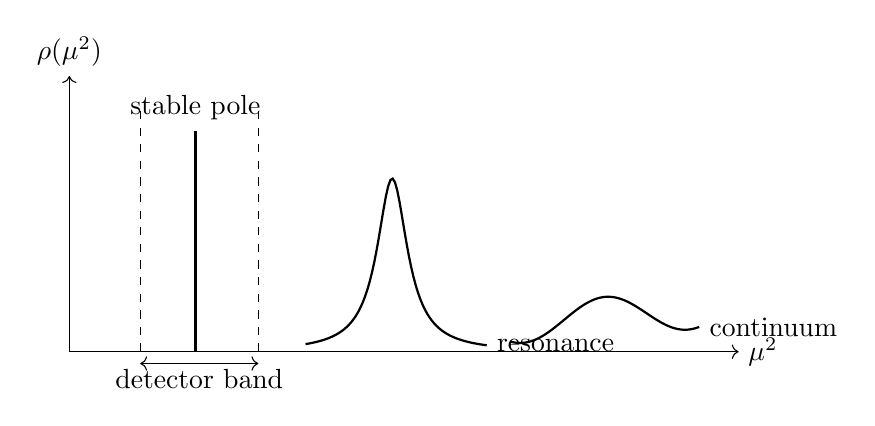
\begin{tikzpicture}[x=1.0cm,y=1.0cm]
    \draw[->] (0,0) -- (8.5,0) node[right] {$\mu^2$};
    \draw[->] (0,0) -- (0,3.5) node[above] {$\rho(\mu^2)$};
    \draw[very thick] (1.6,0) -- (1.6,2.8) node[above] {stable pole};
    \draw[thick,domain=3.0:5.3,samples=80] plot (\x,{2.2/(1+18*(\x-4.1)*(\x-4.1))}) node[right] {resonance};
    \draw[thick,domain=5.6:8.0,samples=100] plot (\x,{0.35+0.25*sin(3*\x r)+0.08*(\x-5.6)}) node[right] {continuum};
    \draw[dashed] (0.9,0) -- (0.9,3.1);
    \draw[dashed] (2.4,0) -- (2.4,3.1);
    \node at (1.65,-0.35) {detector band};
    \draw[<->] (0.9,-0.15) -- (2.4,-0.15);
\end{tikzpicture}
\caption{The same field can contain isolated poles, resonance enhancements, and continua. The functional $\mathcal P_T$ weighs this spectral structure by detector coupling and survival over time.}
\end{figure}

\section{Main properties}

\begin{theorem}[Boundedness]
Assume $\rho\ge0$, $K_D\ge0$, $\Gamma\ge0$, and $0<\int\rho K_D<\infty$. Then
\begin{equation}
0\le \mathcal P_T[\rho,K_D,\Gamma]\le1 .
\end{equation}
\end{theorem}

\begin{proof}
Since $\Gamma\ge0$ and $T\ge0$, $0\le e^{-T\Gamma}\le1$. Multiplying by the nonnegative measure density $\rho K_D$ and integrating gives
\begin{equation}
0\le\int\rho K_D e^{-T\Gamma}\le\int\rho K_D.
\end{equation}
Dividing by the positive denominator proves the claim.
\end{proof}

\begin{theorem}[Monotonicity in observation time]
Under the same assumptions, $\mathcal P_T$ is nonincreasing in $T$.
\end{theorem}

\begin{proof}
For $T_2>T_1$, $e^{-T_2\Gamma}\le e^{-T_1\Gamma}$ pointwise because $\Gamma\ge0$. Integration against the nonnegative weight $\rho K_D$ preserves the inequality. The denominator is independent of $T$.
\end{proof}

\begin{proposition}[Stable-pole limit]
Let
\begin{equation}
\rho(\mu^2)=Z\delta(\mu^2-m^2),\qquad \Gamma(m^2)=0,
\end{equation}
with $ZK_D(m^2)>0$. Then
\begin{equation}
\mathcal P_T=1
\end{equation}
for all $T\ge0$.
\end{proposition}

\begin{proof}
Both numerator and denominator equal $ZK_D(m^2)$ because $e^{-T\Gamma(m^2)}=1$.
\end{proof}

\begin{proposition}[Broad-resonance suppression]
If $\Gamma(\mu^2)\ge\gamma_0>0$ on the support of $\rho K_D$, then
\begin{equation}
\mathcal P_T\le e^{-\gamma_0 T}.
\end{equation}
\end{proposition}

\begin{proof}
On the support of $\rho K_D$, $e^{-T\Gamma}\le e^{-\gamma_0 T}$. Pulling this constant outside the numerator gives the result.
\end{proof}

\section{Relation to real and virtual particles}

This framework does not identify virtual particles with directly detectable particles. Virtual particles are internal terms in perturbative expansions and need not satisfy the on-shell relation $p^2=m^2$. The proposed score applies to spectral support that a detector can couple to. It therefore quantifies \emph{observability of excitation structure}, not literal existence of internal Feynman lines as particles.

The framework can be summarized as follows:
\begin{center}
\begin{tabular}{lll}
\hline
QFT structure & Standard language & Spectral observability view\\
\hline
isolated pole, zero width & stable real particle & $\mathcal P_T\approx1$\\
near pole, small width & unstable particle/resonance & $\mathcal P_T$ high for short $T$\\
broad continuum & multiparticle background & detector-dependent $\mathcal P_T$\\
off-shell internal line & virtual particle & not an asymptotic spectral object\\
\hline
\end{tabular}
\end{center}

\section{Toy model: pole becoming resonance}

Consider a scalar field $\Phi$ coupled to two lighter scalars $\chi$ through
\begin{equation}
\mathcal L=\frac12(\partial\Phi)^2-\frac12M_0^2\Phi^2+\frac12(\partial\chi)^2-\frac12m^2\chi^2-g\Phi\chi^2.
\end{equation}
If $M_0<2m$, decay to two $\chi$ particles is kinematically forbidden and a stable pole may appear below threshold. If the physical mass moves above threshold, the self-energy develops an imaginary part and the excitation becomes unstable.

A schematic resonance spectral density is
\begin{equation}
\rho_R(\mu^2)=\frac{1}{\pi}\frac{M\Gamma}{(\mu^2-M^2)^2+M^2\Gamma^2}.
\end{equation}
If $K_D$ is narrow around $M^2$ and $\Gamma$ is approximately constant, then
\begin{equation}
\mathcal P_T\approx e^{-\Gamma T}.
\end{equation}
Thus the excitation is particle-like on times $T\ll\Gamma^{-1}$ and non-persistent on times $T\gg\Gamma^{-1}$.

\begin{figure}[h]
\centering
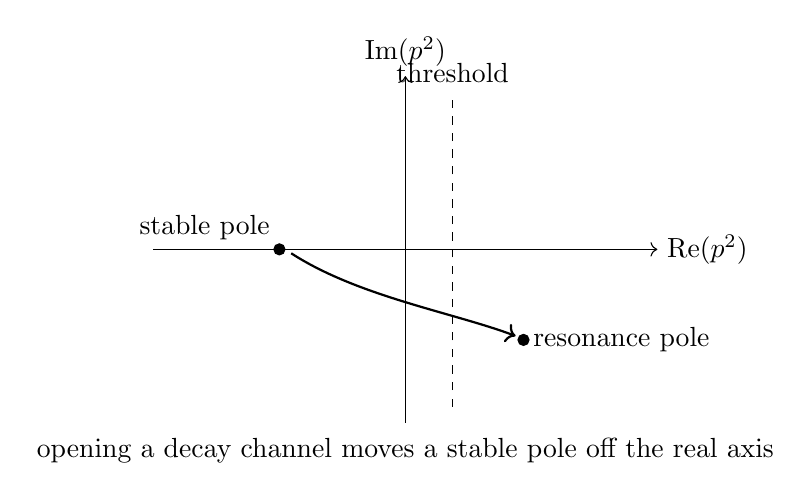
\begin{tikzpicture}[scale=1]
    \draw[->] (-3.2,0) -- (3.2,0) node[right] {$\Re(p^2)$};
    \draw[->] (0,-2.2) -- (0,2.2) node[above] {$\Im(p^2)$};
    \filldraw ( -1.6,0) circle (2pt) node[above left] {stable pole};
    \draw[->,thick] (-1.45,-0.05) .. controls (-0.6,-0.6) and (0.6,-0.8) .. (1.4,-1.1);
    \filldraw (1.5,-1.15) circle (2pt) node[right] {resonance pole};
    \draw[dashed] (0.6,-2) -- (0.6,2) node[above] {threshold};
    \node at (0,-2.55) {opening a decay channel moves a stable pole off the real axis};
\end{tikzpicture}
\caption{A schematic pole migration. The proposed $\mathcal P_T$ score decreases as the effective width increases.}
\end{figure}

\section{Discussion}

The binary vocabulary of ``real'' and ``virtual'' compresses several distinct mathematical facts: on-shellness, asymptotic stability, detector response, lifetime, and spectral isolation. The proposed functional separates these ingredients. A stable LSZ particle remains sharply distinct in the infinite-time limit. But finite experiments operate at finite bandwidth and finite time, where particle-like behavior is naturally graded.

\section{Conclusion}

This paper introduced particle-ness as a normalized spectral observability functional. The main results prove boundedness, monotonicity, the stable-pole limit, and resonance suppression. The framework preserves orthodox QFT while giving a rigorous language for the intuition that field excitations can be more or less particle-like depending on spectral stability and detector coupling.

\begin{thebibliography}{99}

\bibitem{Kallen}
G. K\"allen,
``On the definition of the renormalization constants in quantum electrodynamics,''
\textit{Helvetica Physica Acta} \textbf{25}, 417 (1952).

\bibitem{Lehmann}
H. Lehmann,
``\"Uber Eigenschaften von Ausbreitungsfunktionen und Renormierungskonstanten quantisierter Felder,''
\textit{Nuovo Cimento} \textbf{11}, 342 (1954).

\bibitem{LSZ}
H. Lehmann, K. Symanzik, and W. Zimmermann,
``Zur Formulierung quantisierter Feldtheorien,''
\textit{Nuovo Cimento} \textbf{1}, 205 (1955).

\bibitem{PeskinSchroeder}
M. E. Peskin and D. V. Schroeder,
\textit{An Introduction to Quantum Field Theory}, Addison-Wesley, 1995.

\bibitem{WeinbergQFT}
S. Weinberg,
\textit{The Quantum Theory of Fields, Vol. I}, Cambridge University Press, 1995.

\bibitem{Haag}
R. Haag,
\textit{Local Quantum Physics}, Springer, 1996.

\bibitem{Unruh}
W. G. Unruh,
``Notes on black-hole evaporation,''
\textit{Physical Review D} \textbf{14}, 870 (1976).

\bibitem{DeWitt}
B. S. DeWitt,
``Quantum gravity: the new synthesis,'' in \textit{General Relativity: An Einstein Centenary Survey}, Cambridge University Press, 1979.

\bibitem{Luscher}
M. L\"uscher,
``Signatures of unstable particles in finite volume,''
\textit{Nuclear Physics B} \textbf{364}, 237 (1991).

\bibitem{Ruelle}
D. Ruelle,
``On the asymptotic condition in quantum field theory,''
\textit{Helvetica Physica Acta} \textbf{35}, 147 (1962).

\end{thebibliography}

\end{document}
